%%
%% Class homework & solution template for latex
%% Alex Ihler
%%
\documentclass[twoside,11pt]{article}
\usepackage{amsmath,amsfonts,amssymb,amsthm}
\usepackage{graphicx,color}
\usepackage{verbatim,url}
\usepackage{listings}
\usepackage{hyperref}
\usepackage{upquote}
\usepackage[T1]{fontenc}
%\usepackage{lmodern}
\usepackage[scaled]{beramono}
%\usepackage{textcomp}

% Directories for other source files and images
\newcommand{\bibtexdir}{../bib}
\newcommand{\figdir}{fig}

\newcommand{\E}{\mathrm{E}}
\newcommand{\Var}{\mathrm{Var}}
\newcommand{\N}{\mathcal{N}}
\newcommand{\matlab}{{\sc Matlab}\ }

\setlength{\textheight}{9in} \setlength{\textwidth}{6.5in}
\setlength{\oddsidemargin}{-.25in}  % Centers text.
\setlength{\evensidemargin}{-.25in} %
\setlength{\topmargin}{0in} %
\setlength{\headheight}{0in} %
\setlength{\headsep}{0in} %

\renewcommand{\labelenumi}{(\alph{enumi})}
\renewcommand{\labelenumii}{(\arabic{enumii})}

\theoremstyle{definition}
\newtheorem{MatEx}{M{\scriptsize{ATLAB}} Usage Example}

\definecolor{comments}{rgb}{0,.5,0}
\definecolor{backgnd}{rgb}{.95,.95,.95}
\definecolor{string}{rgb}{.2,.2,.2}
\lstset{language=Matlab}
\lstset{basicstyle=\small\ttfamily,
        mathescape=true,
        emptylines=1, showlines=true,
        backgroundcolor=\color{backgnd},
        commentstyle=\color{comments}\ttfamily, %\rmfamily,
        stringstyle=\color{string}\ttfamily,
        keywordstyle=\ttfamily, %\normalfont,
        showstringspaces=false}
\newcommand{\matp}{\mathbf{\gg}}




\begin{document}

\subsection{Mixed Dimensional Mesh}

Here is an example of applying the heat equation over a simple mixed dimensional mesh. Here is the mesh:
\begin{figure}[h]
\centering
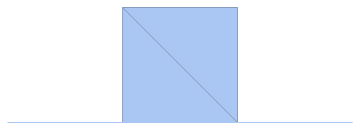
\includegraphics[width=3 in]{mixedMeshPic.png}
\caption{A line and square joined together}
\end{figure}
\\
The topological space has 3 strata: \\
1) The line on the left of the square\\
2) The line on the right of the square\\
3) The square\\
\\
The square can be filtered into its boundary and then the corner points.\\
\\
For the equations below, I will assume it's a line and square. \\
One part of the boundary of the square forms part of the line. 

\subsection{Heat Equation Over Rod}

The heat equation for the rod $u(x,t)$ is as follows:
\[
\alpha_1 \frac{\partial^2 u}{\partial x^2} = \frac{\partial u}{\partial t}
\]
The boundary conditions will be as follows:
\[
u(0,t)=0
\]
\[
u(3,t)=0
\]
The initial condition is as follows:
\[
u(x,0)=-5x(x-3)
\]

\subsection{Heat Equation Over Square}

The square will have a separate heat equation $v(x,y,t)$. \\
Here is the square's diffusion equation:
\[
\alpha_2 (\frac{\partial^2 v}{\partial x^2} + \frac{\partial^2 v}{\partial y^2}) = \frac{\partial v}{\partial t}
\]
The boundary condition on the square will be the values at the rod. Formally this means
\[
v(x,0,t)=u(x,t)
\]
I assumed the square was uniformly heated initially in the y-direction. More formally, 
\[
v(x,y,0)=u(x,0)
\]


\end{document}
